In several contexts, the functional data will present noise, due to the
measurement procedure or to the intrinsic random behaviour of the process,
this will motivate the use of smoothing splines.

\begin{figure}[Example of smoothing]{FIG:SMOOTHING}{Smoothing interpolation}
	\subfigure[SBFIG:SMOOTHING1]{Cubic smoothing}{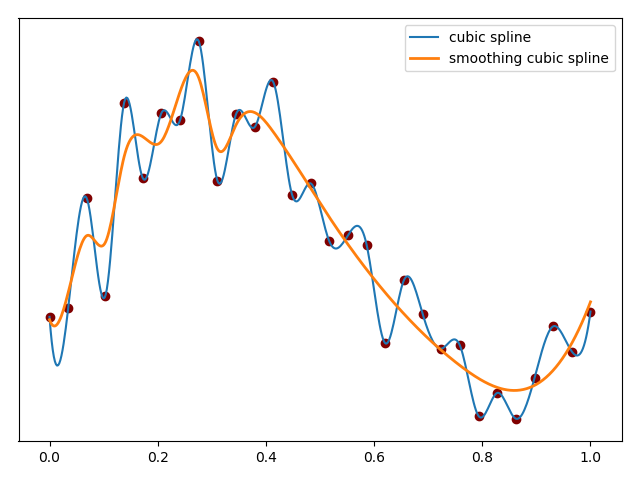
\includegraphics[width=7.5cm]{smoothing-splines}} \quad
	\subfigure[SBFIG:SMOOTHING2]{Several values of the smoothing factor}{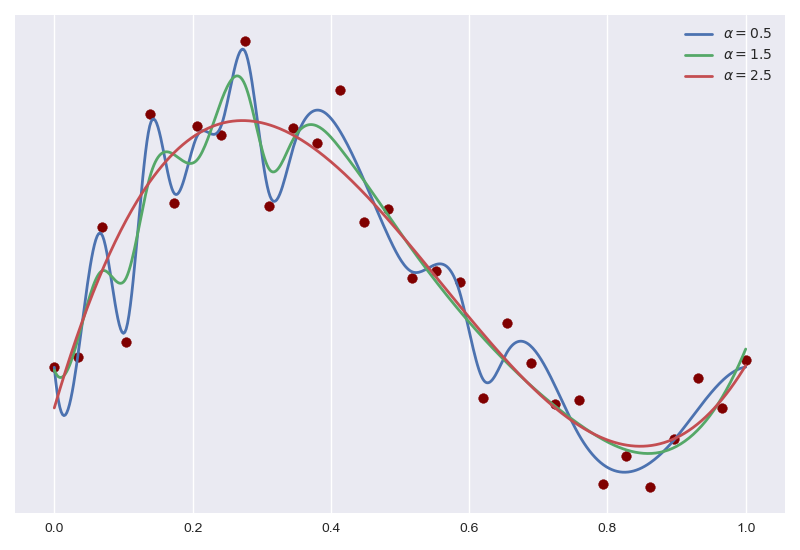
\includegraphics[width=7.5cm]{smoothing-splines-values}}
\end{figure}

This method is a variation of the spline interpolation, but we will not
use directly the points $\{t_k\}_{k=1}^{N}$ as knots. Instead, we will use a
smaller set of knots $\{\tilde t_k\}_{k=1}^{M}$, generally different from the
originals, with their corresponding values $\tilde y_k = x(\tilde t_k)$
calculated using spline interpolation. The function interpolated using smoothing
splines will be defined using spline interpolation on the set of knots
$(\tilde t_k, \tilde y_k)$. Figure \ref{FIG:SMOOTHING} shows the smoothing
interpolation of a noisy observation.


\textcolor{red}{Nexo entre la interpolación y el problema de registration}
